\chapter{Introduction}
\label{chap:introduction}

% The function of this chapter (ca. 2 pages) is to introduce the work, place it for the reader in a context. Often a big problem and after some sub-problems needed to resolve the big one. The introduction leads to a problem statement. After state how this work will tackle the (sub)problem and how (“what is done”). The final paragraph can be guide how the thesis is structured. 


%  
%  
% Main feedback, have a clear structure in this chapter, also guide for further work:

% - Introduce and write for a redear, place the work
% - Work towards a problem statement, based on analysis before. Back up assumptions and motivation by literature.
% - At end, state you aims, link to previous analysis and maybe literature. Here can be specific.




% Main point is to write for the reader, from his/her perspective and turn it to your take on the subject. Back-up statements, how the issue developed by references.

% Paragraph 1, intro to X-ray analysis and why it is important.
Properties of materials are strongly related to their nanoscale composition and structure \cite{callister2014materials}.
The main tool for studying nanoscale structures is the electron microscope (EM), which are divided into scanning electron microscopy (SEM) and transmission electron microscopy (TEM) \cite{goldstein_scanning_2018,williams_carter_tem_2009}.
% The two main tools for studying the nanoscale structure are the scanning and transmission electron microscopes (SEM and TEM). 
The composition at the nanoscale can be studied by analyzing the X-ray spectrum created from the interactions between the material and the electron probe in the EM, thus getting both structural and compositional information \cite{jenkins_xrayspectroscopy}.
The composition is revealed in the X-ray spectrum, where the characteristic lines have energy dependent on the atom of origin, which is a well understood quantum mechanical process \cite{hollas_modern_2004,goldstein_scanning_2018}.
% An X-ray spectrum contains characteristic X-rays lines, a signal from the well understood quantum mechanical process where the energy of the generated X-ray is dependent on the atomic number of the atom that emits the X-ray, revealing the composition of the material \cite{hollas_modern_2004,goldstein_scanning_2018}.
The most common technique for analyzing the X-ray spectrum is energy dispersive X-ray spectroscopy (EDS).
In EDS the electron beam of the microscope excites the material that generates the characteristic X-rays, which are detected and sorted by energy in an accumulating digital histogram.
Even though EDS have limited energy resolution and is affected by several artifacts, it is still the most common technique for analyzing the X-ray spectrum in EM.

% Paragraph 1.5, weakness of XRF and WDS
There are three main techniques in EM for analyzing characteristic X-rays: X-ray fluorescence (XRF), wavelength dispersive spectrometers (WDS), and energy dispersive X-ray spectroscopy \cite{jenkins_xrayspectroscopy}.
In XRF the material is excited by a beam of high-energy X-rays or gamma rays, but the spatial resolution of XRF is limited both by the fact that the beam cannot be focused as thin as the electron beam and that the X-rays can penetrate deeper into the material \cite{xrf_spatial_resolution}.
XRF have some advantages over EDS, such as a very low detection limit and the possibility of being handheld, but the limit in spatial resolution makes it less suitable for EM, thus XRF is therefore not used in this work.
In WDS the material is excited by electrons as in EDS, but the detector has a mechanical spectrometer which is tuned to only one wavelength at a time, that gives a high energy resolution around 10 eV and a high quality spectrum, i.e. a high peak-to-back-ground ratio and limited number of artifacts.
The main issue with WDS is that the setup is much larger than a normal SEM and that the WDS technique is much slower than EDS, usually without the spatial resolution of a SEM \cite{goldstein_scanning_2018}.
Despite the limitations of EDS, the technique is easy to use in EM and gives a high spatial resolution, which makes it the most used analytical technique in research and industry for electron microscopy.





% [Now reader has an intro, and alerted to some weak sides that can be addressed]

% Paragraph 2, introduce the experimental setup characteristics and data treatment that can influence the performance of EDS analysis.
In order to improve the performance of SEM EDS, it is necessary to examine the entire process from signal creation to interpretation, including the data treatment.
By doing so, it becomes possible to identify and address factors that may be responsible for reduced performance.
The EDS signal can be influenced by a range of factors between its creation and detection.
As such, it is important to have a comprehensive understanding of (i) the experimental setup characteristics, (ii) the acquisition parameters, and (iii) the possible post-acquisition data treatment in order to improve the performance of SEM EDS.
This is schematically illustrated in \cref{fig:intro:parameters}.
% (i)
(i) Experimental setup characteristics includes energy resolution in the acquired spectrum, signal-to-noise ratio (SNR) like the Fiori peak-to-background \cite{fiori_peak_background_1982}, detector efficiency, take off angle (TOA), shadowing, and system related artifacts such as strays, all play a crucial role in the quality of the acquired data \cite{goldstein_scanning_2018}.
% Ton did not want: WD, linearity between generation and detection, and stability of resolution and peak positions,
% (ii)
(ii) Similarly, the acquisition parameters affect the spectrum quality and includes parameters like beam energy, probe current, process time, and dwell time. \cite{goldstein_scanning_2018}. % Ton did not want dead time here
Additionally, the (ii) acquisition parameters are somewhat different in SEM and TEM.
TEM samples are typically very thin, at around 100 nm, whereas SEM samples are usually bulk specimens.
Hence, for TEM the SNR can be a limiting factor.
For SEM, addition corrections might be required as signal is created non-uniformly over a larger volume and secondary effects as absorption and fluorescence need to be accounted for.
The beam energy is also different, where TEM is typically operated at 100-300 kV, and SEM is typically operated at 1-30 kV.
The latter energy range is similar to the energy of characteristic X-rays central to this work, and thus the overvoltage effect is significant \cite{williams_carter_companion_volume_2016}.
% (iii)
(iii) Finally, post-acquisition data treatment can have a significant impact on the compositional results.
Post-acquisition data treatment can include making method-specific assumptions, model fitting, and noise treatment \cite{williams_carter_companion_volume_2016}.
Characterization of key parameters is necessary to ensure that a spectrum is acquired correctly, and the detector is operating properly, potentially revealing the need for correction.


% figures/intro_parameters.png
\begin{figure}[!ht]
  \centering
  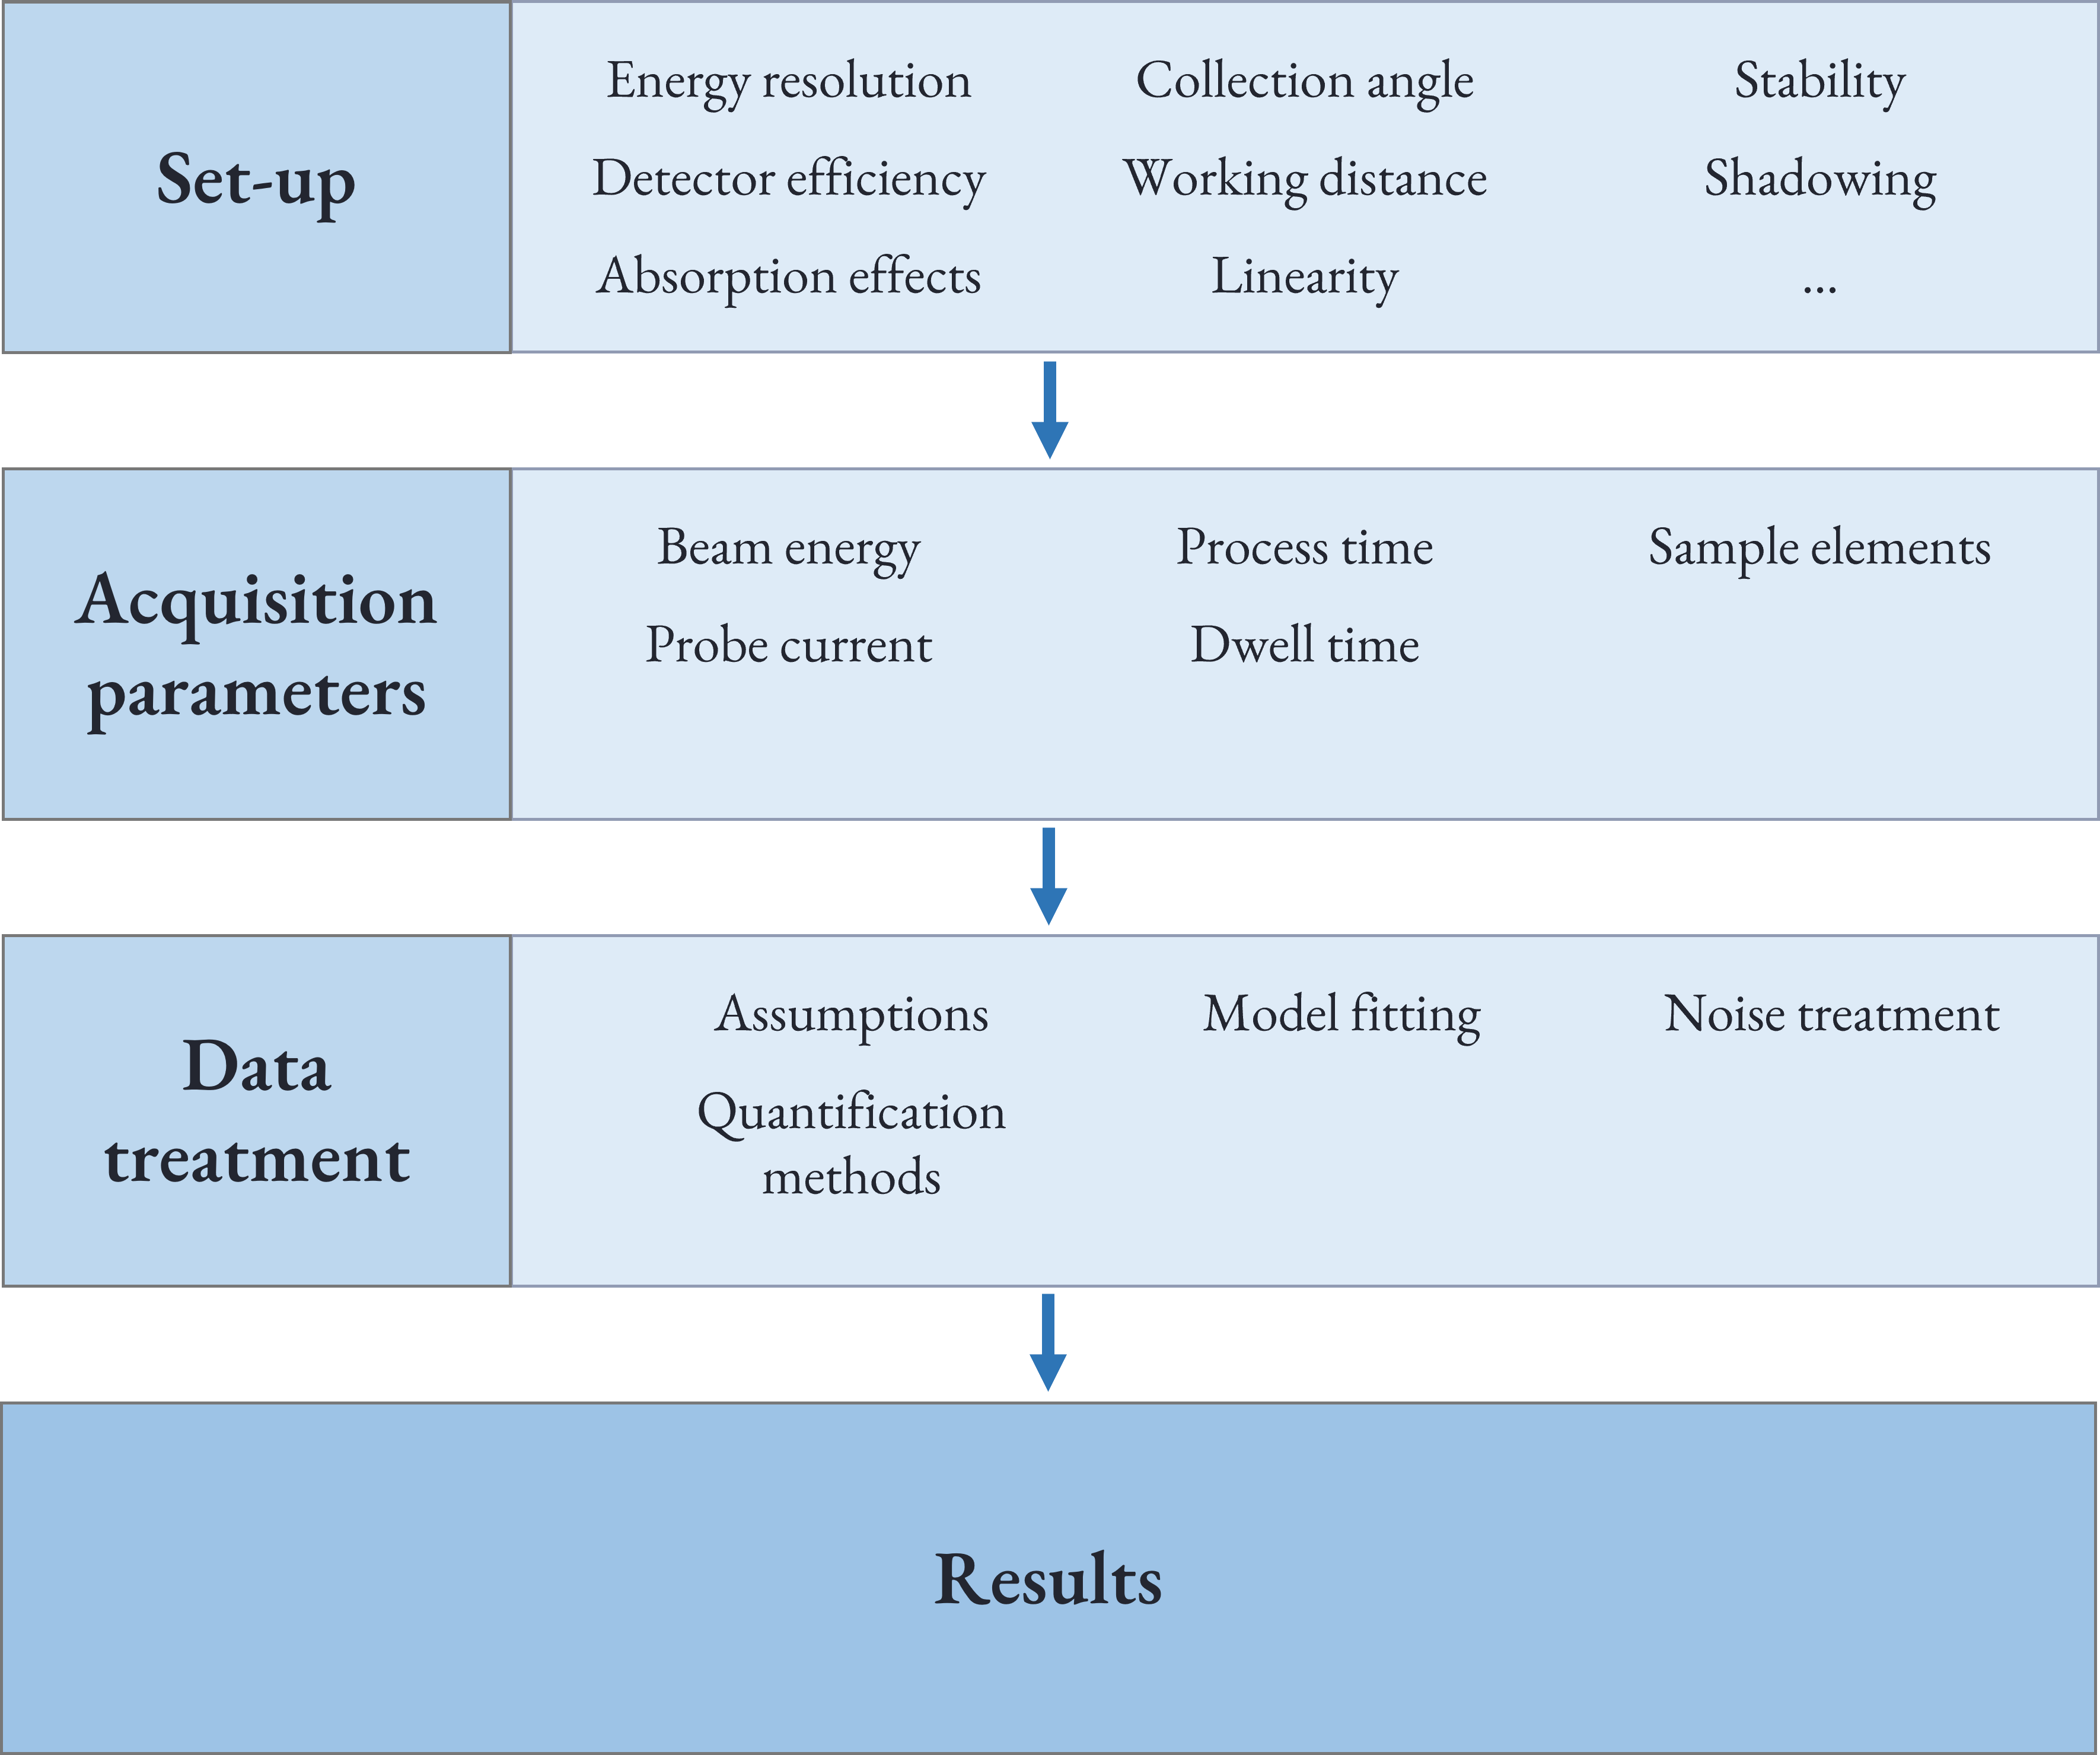
\includegraphics[width=0.8\linewidth]{figures/intro_parameters.png}
  \caption{
    \brynjar{Redo this figure.}
    Schematic illustration of parameters that can affect the performance and results of SEM EDS in the three groups.
    This work focuses on some parameters, with the aim of improving the performance of SEM EDS.
  }
  \label{fig:intro:parameters}
\end{figure}





%%%%%% Paragraph 3: open science and open source software
An additional challenge to improving EDS is that the data treatment in commercial software systems is often not transparent and lacks sufficient open documentation.
This can limit the ability to improve compositional analysis for a given setup and data set.
Typically, only default quantification methods, such as Cliff-Lorimer \cite{CL1975}, are included, while alternative methods, such as optimized correction methods that address weaknesses of default quantification routines and factorless quantification \cite{nilsen_factorless_2021}, are not be available.
In recent years, there has been a growing movement towards open science \cite{opensource_2013}, which has led to an increasing role for open-source tools in EDS analysis.
Community-driven freeware and open-source software have gained importance in the EDS community, for example through the development of open file formats such as .msa and .emsa \cite{iso_emsa_22029} and open source software for data analysis.
For SEM EDS analysis, the main non-commercial software is DTSA-II \cite{dtsaii_1_getting_started}, which is developed at NIST by Nicholas W. M. Ritchie, inspired by the original DTSA microanalysis software developed by Chuck Fiori, Carol Swyt-Thomas, and Bob Myklebust.
For TEM EDS analysis, the Python library HyperSpy \cite{hyperspy_1.7.1} is likely the most used open-source software \brynjar{cite?}.
HyperSpy does have quantification routines implemented, but they are not adapted to SEM EDS signals.
However, HyperSpy has the advantage of being Python-based, which has become a primary programming language for scientific and collaborative work.
Being Python based enables the analyst to benefit from the integration of algorithms from other fields, such as statistics or machine learning, available in Python libraries such as SciPy \cite{2020SciPy}.
Therefore, HyperSpy is a flexible and dynamic platform available for advancing EDS data analysis.





% [Try here to describe your goals and the work that will be done, based on the intro and analysis what is available, and with limitations, as described before. Think first aim is on track, where the second is more ambitious and might need reformulating. Try to be specific and spell out/back-up by references where you go further]


%%%%%%% Paragraph 4: Python notebook for calibration of SEM EDS
% Ton, delete: Electron microscopy plays a vital role in materials characterization in both academic and applied research, and there is still room for improvement in the quantitative analysis of EDS data.
% Ton, delete: To address this, the relevant characteristics of the setup need to be determined.
Earlier work has attempted to improve TEM EDS by making routines for characterizing performance parameters, where a common approach involves analyzing a spectrum of a NiO-thinfilm \cite{egerton_nio_characterization_1994,ted_pella_nio_tem_2019}.
Nylund \cite{nylund_evaluation_2017} and Skomedal \cite{skomedal_improving_2022} have developed a Jupyter notebook to extract characteristics, such as offset and energy resolution \brynjar{list all parameters?}, but even though the reports are available through NTNU Open, the notebooks are not publically available to the electron microscopy community.
Moreover, the notebooks are less suited for lower voltages and bulk samples commonly used in SEM, as Nylund and Skomedal worked with TEM-specimen.
Skomedal worked partly with STEM, showing that the notebook is relevant for lower voltages, but the effect of bulk samples is not addressed, which will be addressed in this work.
Reference values for characteristics like Fiori P/B, \brynjar{parameter 2, and parameter 3 (with citation)} are available in the literature, but the values are specified for older Si(Li) type of EDS detectors and may not apply to modern silicon drift detectors (SDDs) \cite{sdd_lechner_2001}.
To fill this gap, a Python notebook for characterization of performance parameters in a SEM EDS setup will be developed and published, including transparent documentation.
The main focus will be SEM EDS, but the notebook should also be applicable to TEM EDS.
Following the notebook will be a proposition for a SEM EDS tailored test specimen.
This work will contribute to improving the EDS setup and acquisition of EDS data, which will aid the quantitative analysis of EDS data, and hence advance the field of materials science.
\ton{Say something about what area of science this is most relevant for? E.g. not biology.}



%%%%%%% Paragraph 5: the more hairy goal of adding bulk quantification to HyperSpy
% A second, more ambitious, goal 
The overall aim, as stated by the project title, is to improve EDS.
The first goal is to systematically go through the parameter listed in \cref{fig:intro:parameters}, and characterize the performance of a SEM EDS setup.
The main focus will be on the experimental characteristics and new data processing routines that become available through open-source packages.
The second goal is to develop open-source software for bulk quantification of EDS data, as an addition to the HyperSpy package.
The default approach for bulk is a ratio approach with a sensitivity factor, as for the now implemented Cliff-Lorimer-ratio method that is accepted for thin specimen geometries as used in TEM, but bulk specimen needs an iterative and model-based correction routine for atomic number (Z), absorption (A) and fluorescence (F) \cite{goldstein_scanning_2018}.
Alternatively, the Phi-Rho-Z quantification method can correct for the bulk effects \brynjar{cite}.
Neither the ZAF nor Phi-Rho-Z-corrections are implemented in HyperSpy, where the quantification analysis utilize the thin-film approximation.
Other methods like the factorless internal composition determination \cite{nilsen_factorless_2021} \ton{is this correctly phrased?} can also be used for quantification.
This work aims to explore whether iterative ZAF or Z Phi-Rho-Z-corrections can be implemented in the HyperSpy environment, to allow quantification in the low energy range for bulk specimen.




Last paragraph will be a guide how the report is build up, as in the project report. Added later.









